% Gráfico: Ordenação - Média de Nós Restantes
\begin{figure}[htbp]
\centering
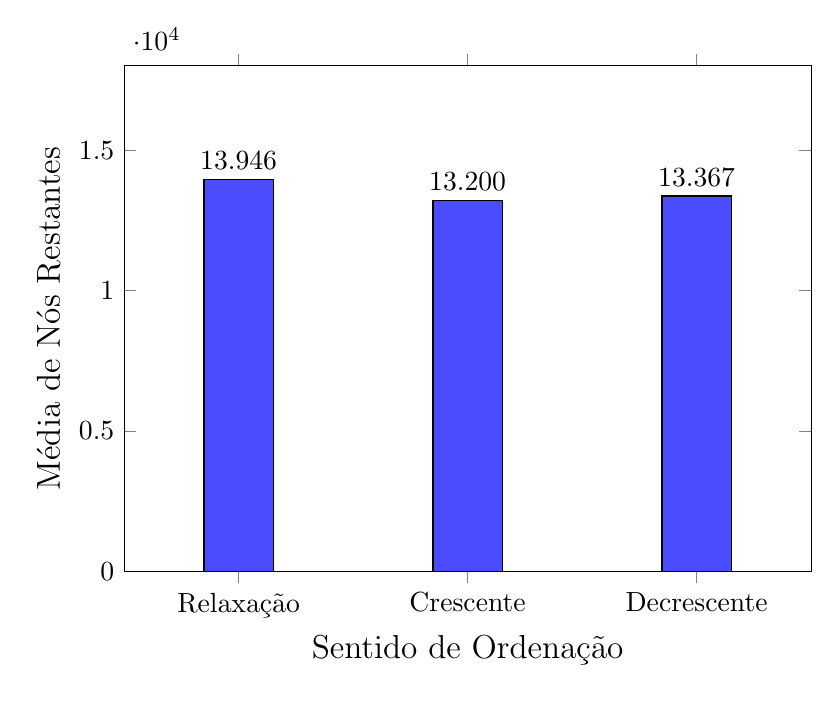
\begin{tikzpicture}
\begin{axis}[
    ybar,
    bar width=25pt,
    width=0.85\textwidth,
    height=8cm,
    ylabel={Média de Nós Restantes},
    xlabel={Sentido de Ordenação},
    symbolic x coords={Relaxação, Crescente, Decrescente},
    xtick=data,
    nodes near coords,
    nodes near coords align={vertical},
    nodes near coords style={font=\normalsize},
    every node near coord/.append style={/pgf/number format/fixed,
        /pgf/number format/precision=0,
        /pgf/number format/use comma},
    ymin=0,
    ymax=18000,
    enlarge x limits=0.25,
    ylabel style={font=\large},
    xlabel style={font=\large},
    tick label style={font=\normalsize},
]
\addplot[fill=blue!70] coordinates {
    (Relaxação,13946)
    (Crescente,13200)
    (Decrescente,13367)
};
\end{axis}
\end{tikzpicture}
\caption{Média de nós restantes por instância comparando ordenação crescente e decrescente. A ordenação crescente obteve a menor média, com 13.200 nós restantes.}
\label{fig:avg_nodes_order}
\end{figure}
